% The Newton–Schulz map of Section 2.3.2: what one step and five steps do to a singular value of the normalized matrix, on a logarithmic axis. The coordinates were computed from the coefficients of the text.
\definecolor{moeblue}{RGB}{49,101,156}
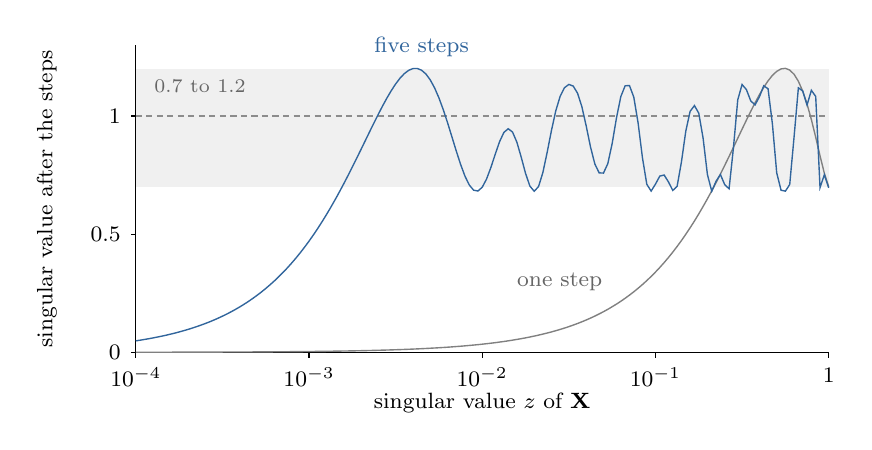
\begin{tikzpicture}[x=2.2cm, y=3.0cm, font=\footnotesize, line width=0.5pt]
  % The band the text mentions, and the value one.
  \fill[black!6] (-4, 0.7) rectangle (0, 1.2);
  \draw[black!45, dashed, dash pattern=on 2.2pt off 1.6pt] (-4, 1) -- (0, 1);
  \node[anchor=west, text=black!60, font=\scriptsize] at (-3.95, 1.125) {0.7 to 1.2};
  % Axes.
  \draw (-4, 0) -- (0, 0);
  \draw (-4, 0) -- (-4, 1.3);
  \foreach \x/\t in {-4/$10^{-4}$, -3/$10^{-3}$, -2/$10^{-2}$, -1/$10^{-1}$, 0/$1$} {
    \draw (\x, 0) -- (\x, -0.025) node[below] {\t};
  }
  \foreach \y/\t in {0/$0$, 0.5/$0.5$, 1/$1$} {
    \draw (-4, \y) -- (-4.03, \y) node[left] {\t};
  }
  \node[below] at (-2, -0.13) {singular value $z$ of $\mathbf{X}$};
  \node[rotate=90, anchor=south] at (-4.4, 0.65) {singular value after the steps};
  % Curves.
  \draw[black!50] plot coordinates {(-4.000,0.0003) (-3.975,0.0004) (-3.950,0.0004) (-3.925,0.0004) (-3.900,0.0004) (-3.875,0.0005) (-3.850,0.0005) (-3.825,0.0005) (-3.800,0.0005) (-3.775,0.0006) (-3.750,0.0006) (-3.725,0.0006) (-3.700,0.0007) (-3.675,0.0007) (-3.650,0.0008) (-3.625,0.0008) (-3.600,0.0009) (-3.575,0.0009) (-3.550,0.0010) (-3.525,0.0010) (-3.500,0.0011) (-3.475,0.0012) (-3.450,0.0012) (-3.425,0.0013) (-3.400,0.0014) (-3.375,0.0015) (-3.350,0.0015) (-3.325,0.0016) (-3.300,0.0017) (-3.275,0.0018) (-3.250,0.0019) (-3.225,0.0021) (-3.200,0.0022) (-3.175,0.0023) (-3.150,0.0024) (-3.125,0.0026) (-3.100,0.0027) (-3.075,0.0029) (-3.050,0.0031) (-3.025,0.0033) (-3.000,0.0034) (-2.975,0.0036) (-2.950,0.0039) (-2.925,0.0041) (-2.900,0.0043) (-2.875,0.0046) (-2.850,0.0049) (-2.825,0.0052) (-2.800,0.0055) (-2.775,0.0058) (-2.750,0.0061) (-2.725,0.0065) (-2.700,0.0069) (-2.675,0.0073) (-2.650,0.0077) (-2.625,0.0082) (-2.600,0.0087) (-2.575,0.0092) (-2.550,0.0097) (-2.525,0.0103) (-2.500,0.0109) (-2.475,0.0115) (-2.450,0.0122) (-2.425,0.0129) (-2.400,0.0137) (-2.375,0.0145) (-2.350,0.0154) (-2.325,0.0163) (-2.300,0.0173) (-2.275,0.0183) (-2.250,0.0194) (-2.225,0.0205) (-2.200,0.0217) (-2.175,0.0230) (-2.150,0.0244) (-2.125,0.0258) (-2.100,0.0274) (-2.075,0.0290) (-2.050,0.0307) (-2.025,0.0325) (-2.000,0.0344) (-1.975,0.0365) (-1.950,0.0386) (-1.925,0.0409) (-1.900,0.0434) (-1.875,0.0459) (-1.850,0.0486) (-1.825,0.0515) (-1.800,0.0546) (-1.775,0.0578) (-1.750,0.0612) (-1.725,0.0649) (-1.700,0.0687) (-1.675,0.0728) (-1.650,0.0771) (-1.625,0.0816) (-1.600,0.0864) (-1.575,0.0916) (-1.550,0.0970) (-1.525,0.1027) (-1.500,0.1088) (-1.475,0.1152) (-1.450,0.1220) (-1.425,0.1292) (-1.400,0.1368) (-1.375,0.1449) (-1.350,0.1534) (-1.325,0.1625) (-1.300,0.1720) (-1.275,0.1821) (-1.250,0.1929) (-1.225,0.2042) (-1.200,0.2161) (-1.175,0.2288) (-1.150,0.2422) (-1.125,0.2563) (-1.100,0.2712) (-1.075,0.2870) (-1.050,0.3036) (-1.025,0.3212) (-1.000,0.3397) (-0.975,0.3592) (-0.950,0.3798) (-0.925,0.4014) (-0.900,0.4242) (-0.875,0.4481) (-0.850,0.4732) (-0.825,0.4995) (-0.800,0.5271) (-0.775,0.5559) (-0.750,0.5860) (-0.725,0.6174) (-0.700,0.6500) (-0.675,0.6838) (-0.650,0.7187) (-0.625,0.7547) (-0.600,0.7916) (-0.575,0.8293) (-0.550,0.8675) (-0.525,0.9061) (-0.500,0.9447) (-0.475,0.9829) (-0.450,1.0203) (-0.425,1.0563) (-0.400,1.0903) (-0.375,1.1215) (-0.350,1.1492) (-0.325,1.1722) (-0.300,1.1894) (-0.275,1.1998) (-0.250,1.2021) (-0.225,1.1949) (-0.200,1.1771) (-0.175,1.1475) (-0.150,1.1055) (-0.125,1.0512) (-0.100,0.9853) (-0.075,0.9106) (-0.050,0.8319) (-0.025,0.7576) (0.000,0.7010)};
  \draw[moeblue] plot coordinates {(-4.000,0.0485) (-3.975,0.0513) (-3.950,0.0544) (-3.925,0.0576) (-3.900,0.0610) (-3.875,0.0646) (-3.850,0.0684) (-3.825,0.0725) (-3.800,0.0768) (-3.775,0.0813) (-3.750,0.0861) (-3.725,0.0912) (-3.700,0.0966) (-3.675,0.1023) (-3.650,0.1084) (-3.625,0.1148) (-3.600,0.1216) (-3.575,0.1287) (-3.550,0.1363) (-3.525,0.1444) (-3.500,0.1529) (-3.475,0.1619) (-3.450,0.1714) (-3.425,0.1815) (-3.400,0.1921) (-3.375,0.2034) (-3.350,0.2153) (-3.325,0.2279) (-3.300,0.2412) (-3.275,0.2552) (-3.250,0.2701) (-3.225,0.2858) (-3.200,0.3023) (-3.175,0.3198) (-3.150,0.3381) (-3.125,0.3575) (-3.100,0.3779) (-3.075,0.3994) (-3.050,0.4220) (-3.025,0.4457) (-3.000,0.4705) (-2.975,0.4966) (-2.950,0.5239) (-2.925,0.5524) (-2.900,0.5821) (-2.875,0.6130) (-2.850,0.6451) (-2.825,0.6783) (-2.800,0.7127) (-2.775,0.7480) (-2.750,0.7842) (-2.725,0.8211) (-2.700,0.8585) (-2.675,0.8962) (-2.650,0.9339) (-2.625,0.9712) (-2.600,1.0078) (-2.575,1.0432) (-2.550,1.0767) (-2.525,1.1078) (-2.500,1.1359) (-2.475,1.1601) (-2.450,1.1796) (-2.425,1.1936) (-2.400,1.2012) (-2.375,1.2016) (-2.350,1.1941) (-2.325,1.1781) (-2.300,1.1532) (-2.275,1.1194) (-2.250,1.0771) (-2.225,1.0273) (-2.200,0.9716) (-2.175,0.9123) (-2.150,0.8525) (-2.125,0.7958) (-2.100,0.7464) (-2.075,0.7086) (-2.050,0.6865) (-2.025,0.6828) (-2.000,0.6989) (-1.975,0.7336) (-1.950,0.7826) (-1.925,0.8385) (-1.900,0.8916) (-1.875,0.9309) (-1.850,0.9465) (-1.825,0.9325) (-1.800,0.8895) (-1.775,0.8261) (-1.750,0.7577) (-1.725,0.7038) (-1.700,0.6819) (-1.675,0.7016) (-1.650,0.7610) (-1.625,0.8472) (-1.600,0.9407) (-1.575,1.0235) (-1.550,1.0843) (-1.525,1.1203) (-1.500,1.1341) (-1.475,1.1272) (-1.450,1.0974) (-1.425,1.0403) (-1.400,0.9588) (-1.375,0.8695) (-1.350,0.7976) (-1.325,0.7596) (-1.300,0.7588) (-1.275,0.7990) (-1.250,0.8837) (-1.225,0.9924) (-1.200,1.0826) (-1.175,1.1285) (-1.150,1.1291) (-1.125,1.0800) (-1.100,0.9697) (-1.075,0.8231) (-1.050,0.7114) (-1.025,0.6825) (-1.000,0.7121) (-0.975,0.7459) (-0.950,0.7506) (-0.925,0.7214) (-0.900,0.6852) (-0.875,0.7027) (-0.850,0.8061) (-0.825,0.9359) (-0.800,1.0200) (-0.775,1.0446) (-0.750,1.0123) (-0.725,0.9065) (-0.700,0.7523) (-0.675,0.6819) (-0.650,0.7246) (-0.625,0.7526) (-0.600,0.7094) (-0.575,0.6923) (-0.550,0.8648) (-0.525,1.0688) (-0.500,1.1337) (-0.475,1.1121) (-0.450,1.0644) (-0.425,1.0475) (-0.400,1.0816) (-0.375,1.1283) (-0.350,1.1156) (-0.325,0.9674) (-0.300,0.7591) (-0.275,0.6863) (-0.250,0.6823) (-0.225,0.7104) (-0.200,0.9104) (-0.175,1.1197) (-0.150,1.1065) (-0.125,1.0467) (-0.100,1.1092) (-0.075,1.0833) (-0.050,0.6975) (-0.025,0.7516) (0.000,0.6964)};
  \node[text=black!60, anchor=east] at (-1.25, 0.3) {one step};
  \node[text=moeblue, anchor=south] at (-2.35, 1.21) {five steps};
\end{tikzpicture}
